\chapter{Pembuatan \textit{Virtual Machine} (VM) pada DigitalOcean}
\label{appendix:A}

Langkah-langkah pembuatan VM pada DigitalOcean dijelaskan seperti berikut,
\begin{enumerate}
  \item Buatlah akun DigitalOcean terlebih dahulu. Jika belum memiliki akun DigitalOcean, disarankan untuk mendaftar melalui \textit{GitHub Student Developer Pack} sehingga nantinya akan diberikan kredit \$200 secara gratis. Jika sudah memiliki akun DigitalOcean, silakan melakukan \textit{login}.
  \item Halaman dasbor DigitalOcean akan ditampilkan setelahnya.
	\begin{center}
	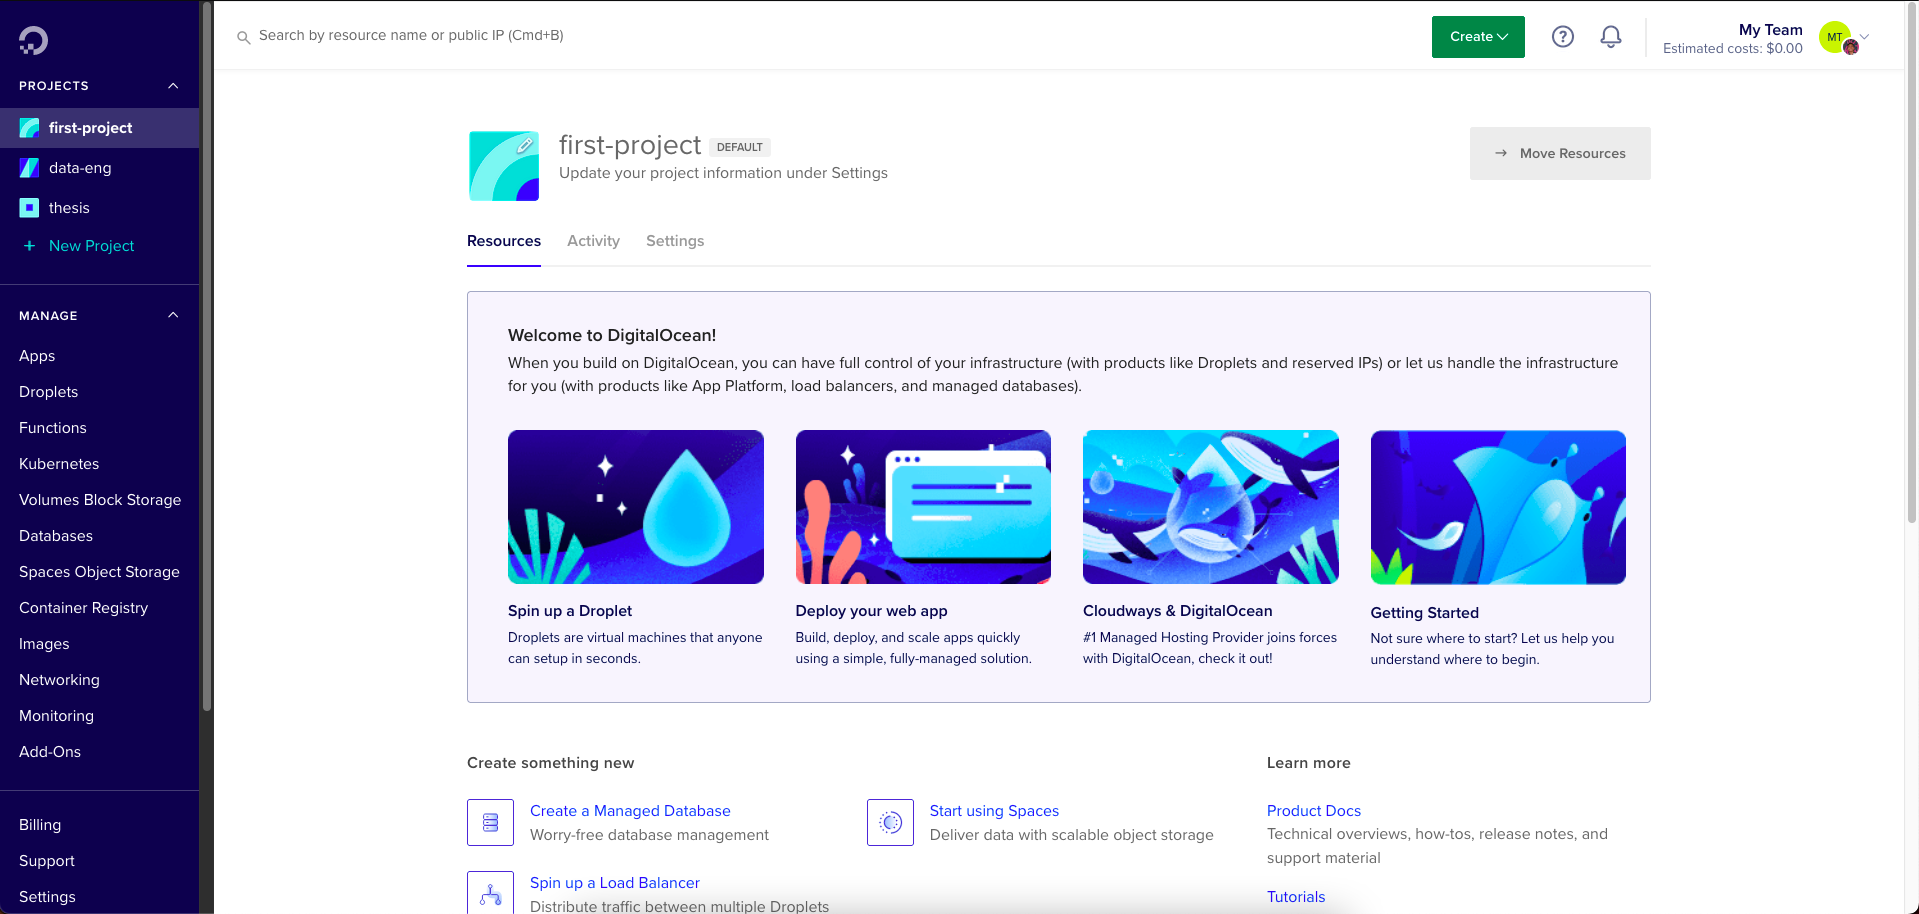
\includegraphics[width=1\linewidth]{figures/ch99/ap1/1.png}
	\end{center} 
  \item Perhatikan menu di sebelah kiri pada laman dasbor DigitalOcean. Tekan Droplets untuk masuk ke laman pembuatan VM. Selanjutnya, tekan \textit{Create Droplets} berwarna biru untuk melakukan konfigurasi VM yang akan dibuat nantinya. \pagebreak
	\begin{center}
	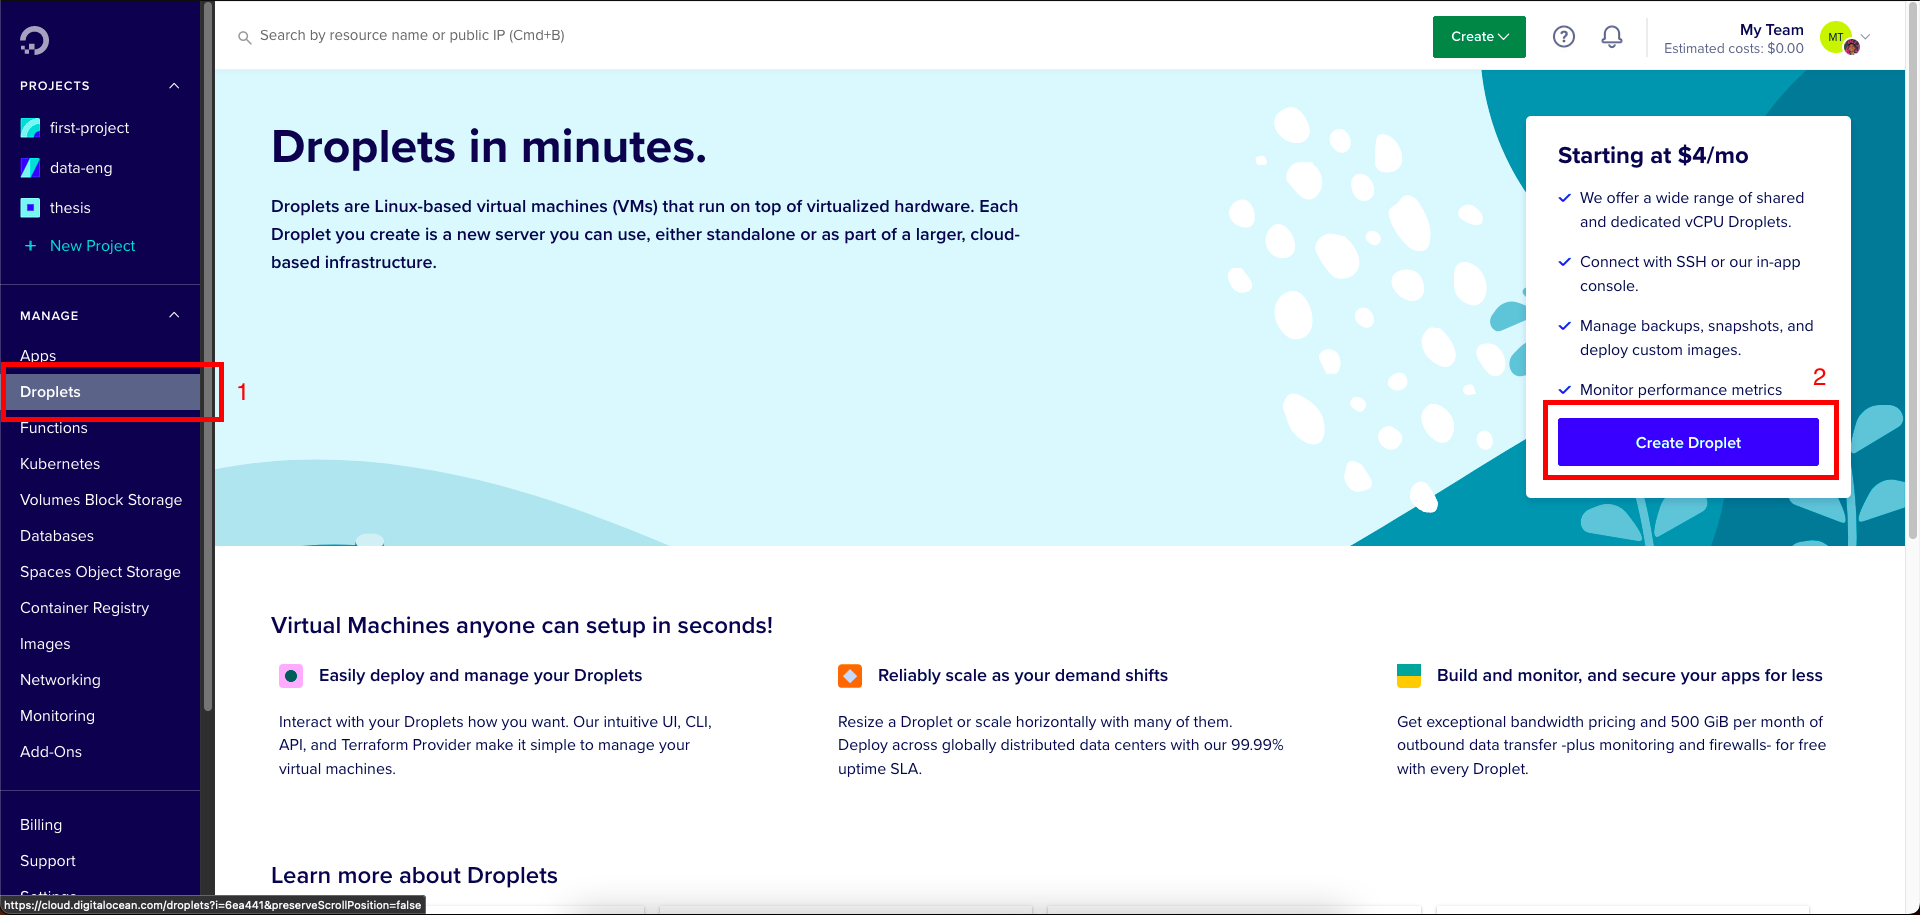
\includegraphics[width=1\linewidth]{figures/ch99/ap1/2.png}
	\end{center} 
  \item Pada laman pembuatan Droplets, lakukan konfigurasi sesuai dengan Tabel \ref{table:conf-hardware}. Jika telah selesai melakukan konfigurasi, tekan \textit{Create Droplets}. 
	\begin{center}
	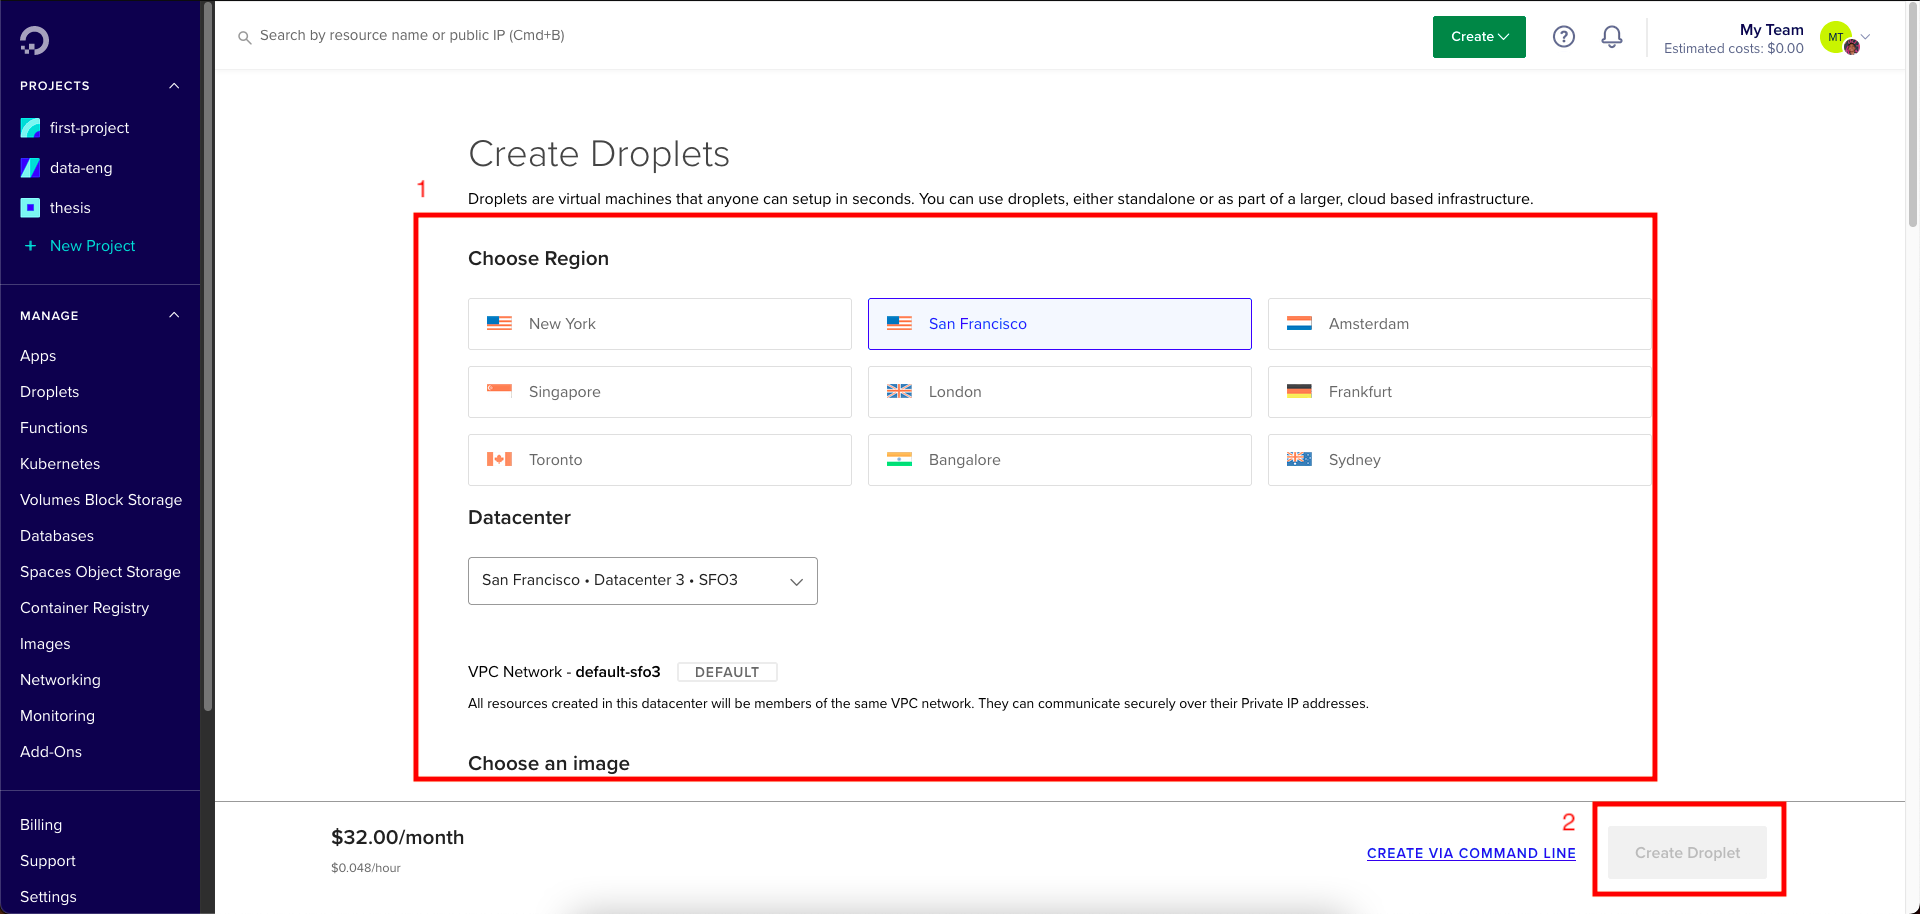
\includegraphics[width=1\linewidth]{figures/ch99/ap1/3.png}
	\end{center} 
  \item Jika pembuatan Droplets berhasil, laman dasbor \textit{Projects} DigitalOcean akan terlihat. Pada bagian Resources akan terlihat Droplets yang baru saja kita buat. Selanjutnya, tekan nama Droplets yang baru saja dibuat. 
	\begin{center}
	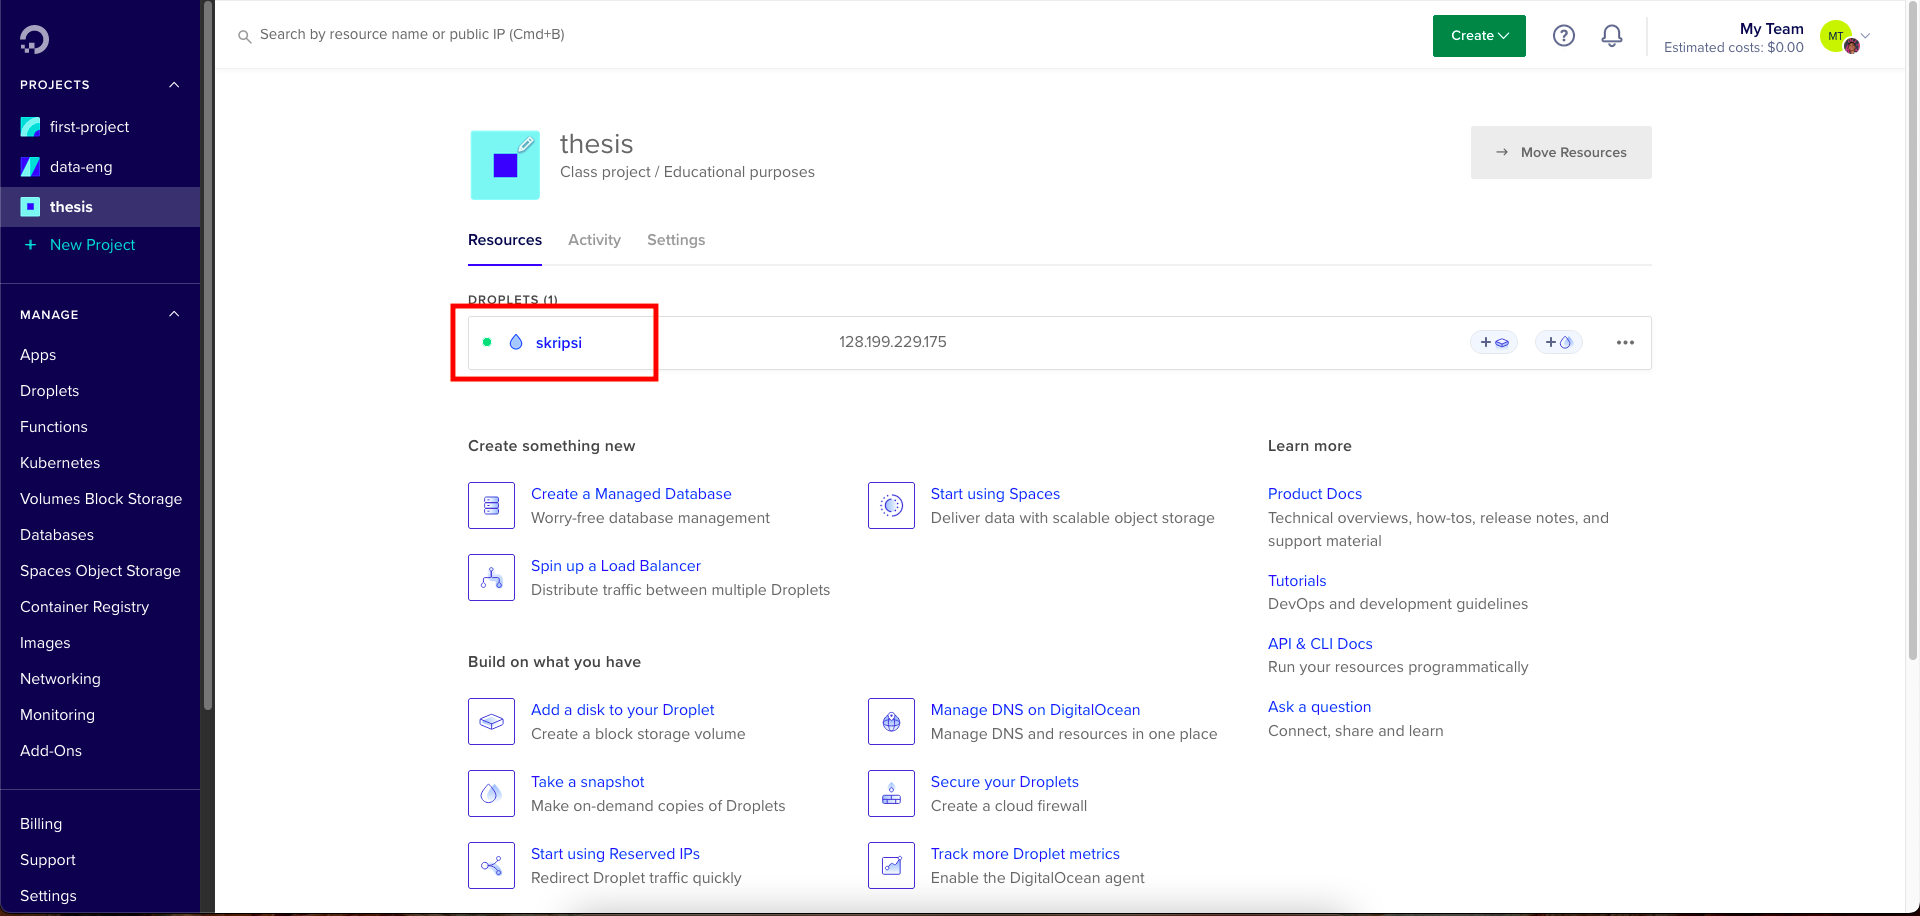
\includegraphics[width=1\linewidth]{figures/ch99/ap1/4.png}
	\end{center} 
  \item Selanjutnya, laman konfigurasi Droplets akan terlihat. Jika diperlukan konfigurasi lanjutan dapat diatur melalui laman ini. Pada tahap ini hanya akan fokus pada konfigurasi perangkat lunak tanpa konfigurasi perangkat keras lebih jauh. Untuk masuk ke VM yang sudah dibuat, tekan Console. \textit{Tab} baru akan dibuka.
	\begin{center}
	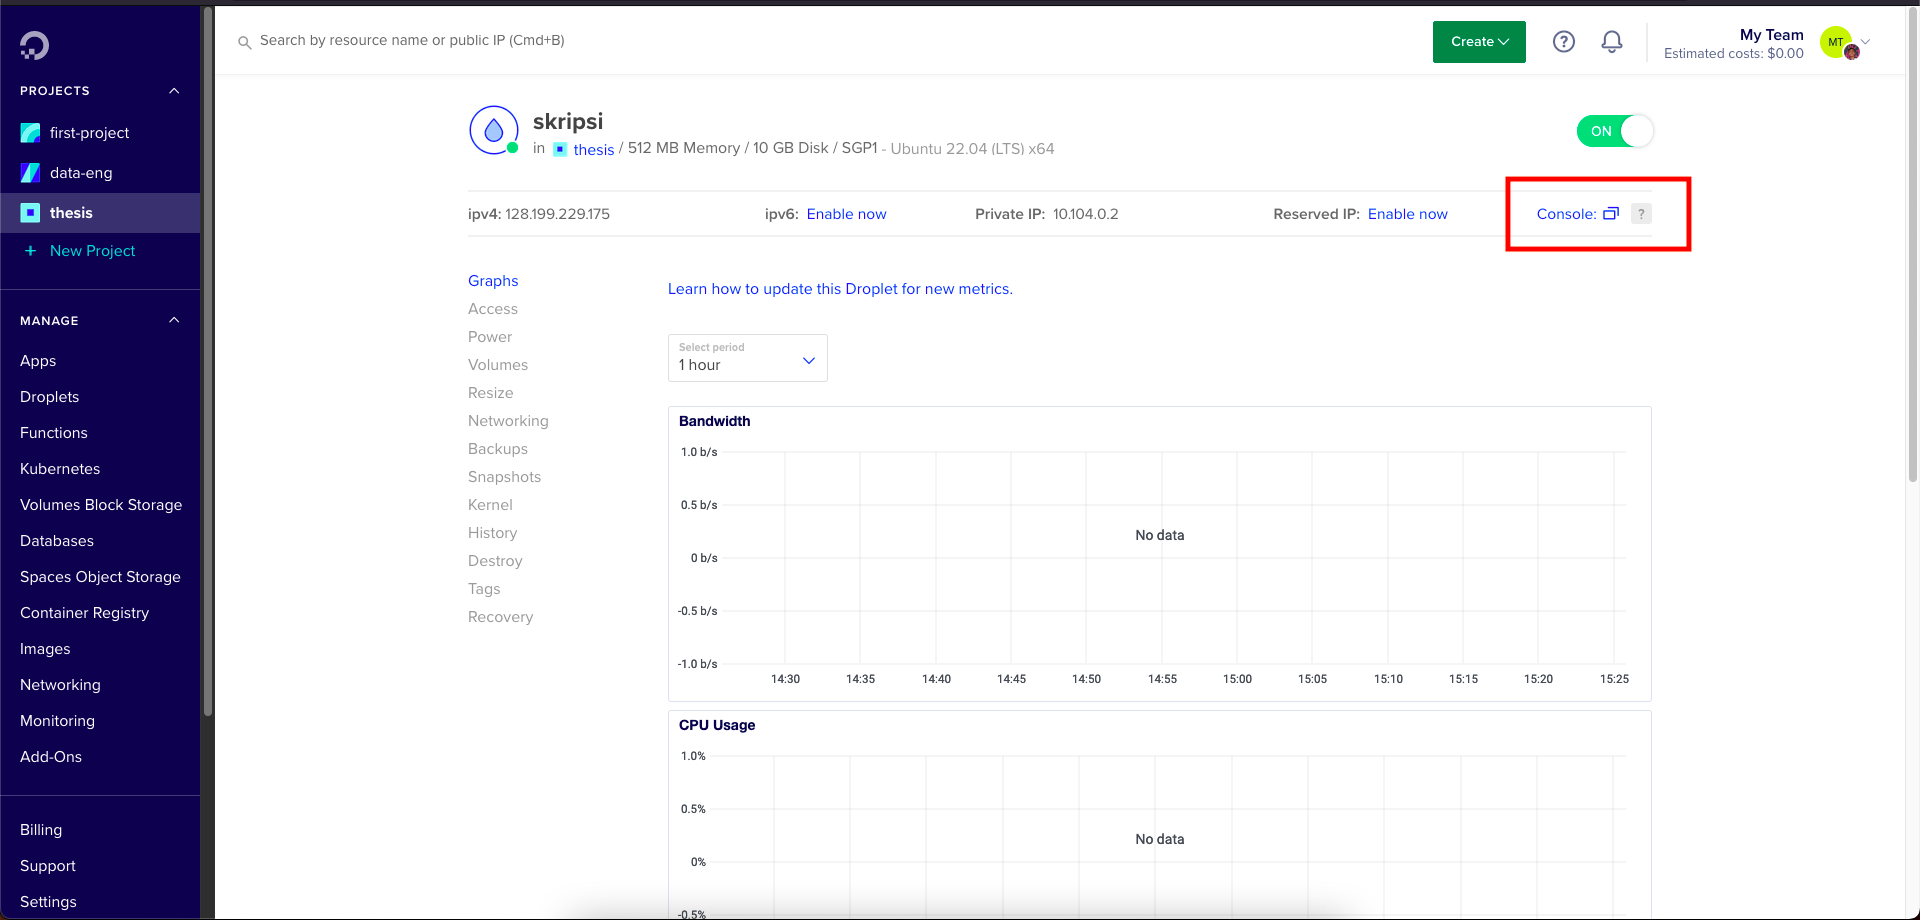
\includegraphics[width=1\linewidth]{figures/ch99/ap1/5.png}
	\end{center} 
  \item Akhirnya, lakukan konfigurasi perangkat lunak pada bagian ini.
	\begin{center}
	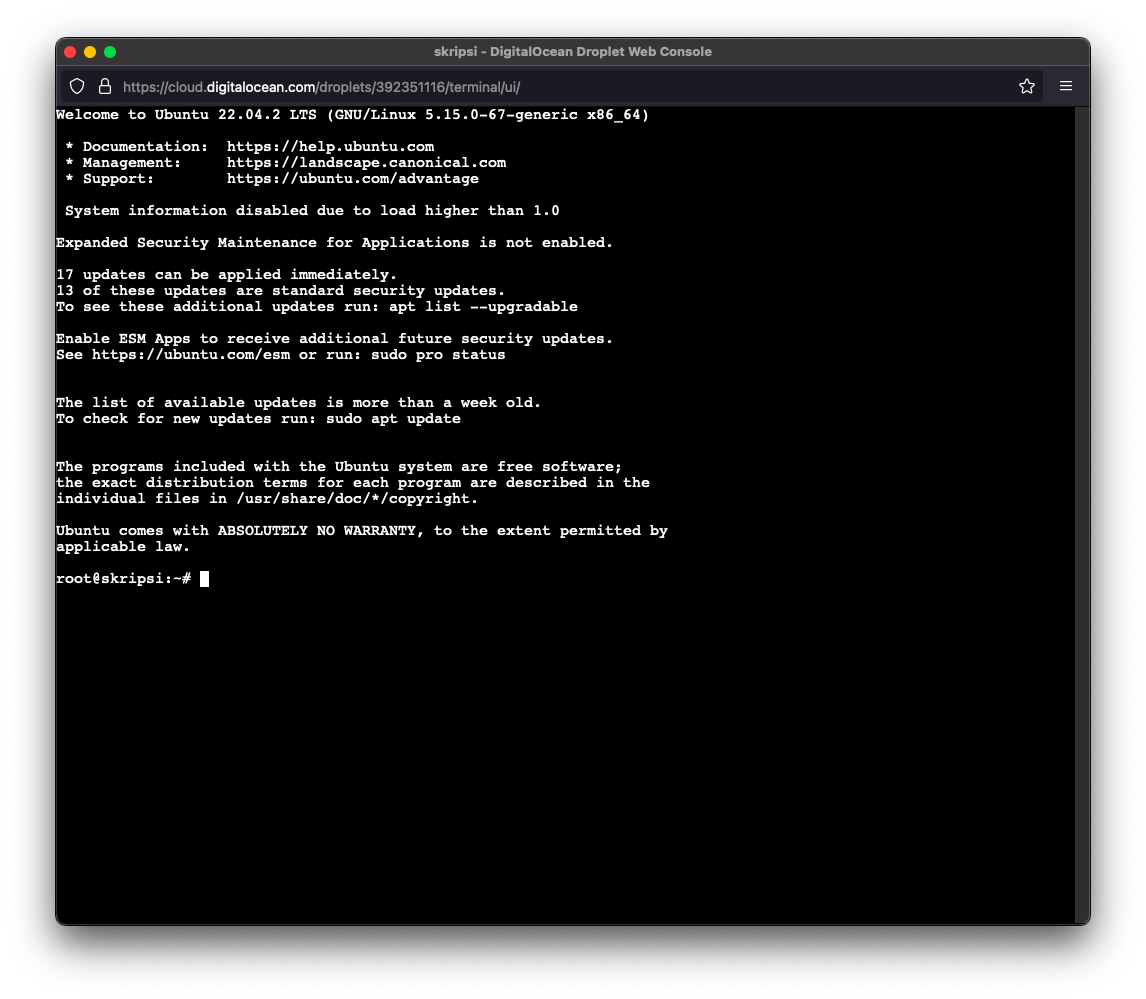
\includegraphics[width=1\linewidth]{figures/ch99/ap1/6.png}
	\end{center} 

\end{enumerate}